\section{開発フロー}
DNNのHWアクセラレーションには,Xilinx社から提供されているDPU(Deeplearning Processing Unit)コア\cite{dpuip}および統合開発環境であるVitis-AIを使用した.
Vitis-AIはcaffe,tensorflow等のDNNフレームワークを用いて設計されたDNNモデルを量子化し,DPU向けにデプロイすることができる.\footnote{Vitis-AI v1.3にてpytorchへの一部対応が追加された.}
\section{DNNモデルの学習}
\subsection{DNNモデル}
コンテストの課題であるセマンティックセグメンテーションを行うDNNモデルとして我々はresnet18-FPNを使用した.
モデルはXilinx社から提供されるチュートリアル\cite{tutorial}に含まれるものを流用した.
FPN(Feature Pyramid Network)\cite{fpn}は,低解像だが意味的に強い(semantically strong)特徴と高解像だが意味的に弱い(semantically weak)特徴の両方を使用することで物体検出及び領域分割のタスクにおいて高い精度を挙げられることが知られている.図\ref{figure_fpn}にFPNの概要図を示す.
\begin{figure}[t]
    \begin{center}
        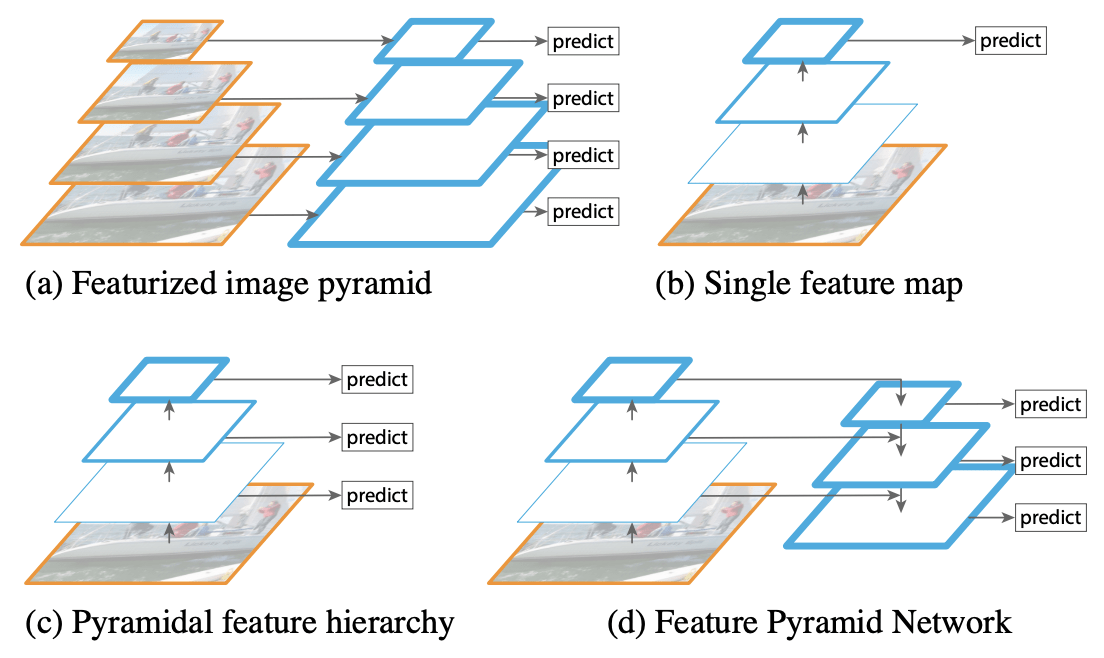
\includegraphics[width=8.0cm]{figures/fpn.png}
        \caption{Feature Pyramid Network\cite{fpn}}
        \label{figure_fpn}
        \end{center}
\end{figure}
\subsection{損失関数}
参考にしたチュートリアルでは損失関数としてSoftmaxWithCrossEntropyが使用されていた.コンテストで提供される学習画像を使用して学習を行ったが,テスト画像に対するmIoUスコアは0.50程度に留まり,処理速度部門における基準値である0.60を上回ることができなかった.
そこで我々は領域分割タスクにおいて精度を向上させる損失関数として提案されているLovasz-Loss関数\cite{lovasz}を採用した.Lovasz-Loss関数は,第1回AIエッジコンテストのセグメンテーション部門において第2位のチームも使用していたことから\cite{ref_signate_report},精度向上に効果的であると考えた.
Lovasz-Lossは予測領域と正解領域のIoUを指標とするJaccard-Lossをさらに拡張したものであり,tensorflowとpytorch向けに公式に実装が公開されている.流用したチュートリアルはCaffeを用いてモデルが定義されており,Caffe上でLovasz-Loss関数を自前で実装するのは困難であった.モデルをpytorchに変換してpytorch上で学習を行い,学習済みの重みをcaffe向けに変換することでこの問題を解消した.
\subsection{学習結果}
\begin{figure}[t]
    \begin{center}
        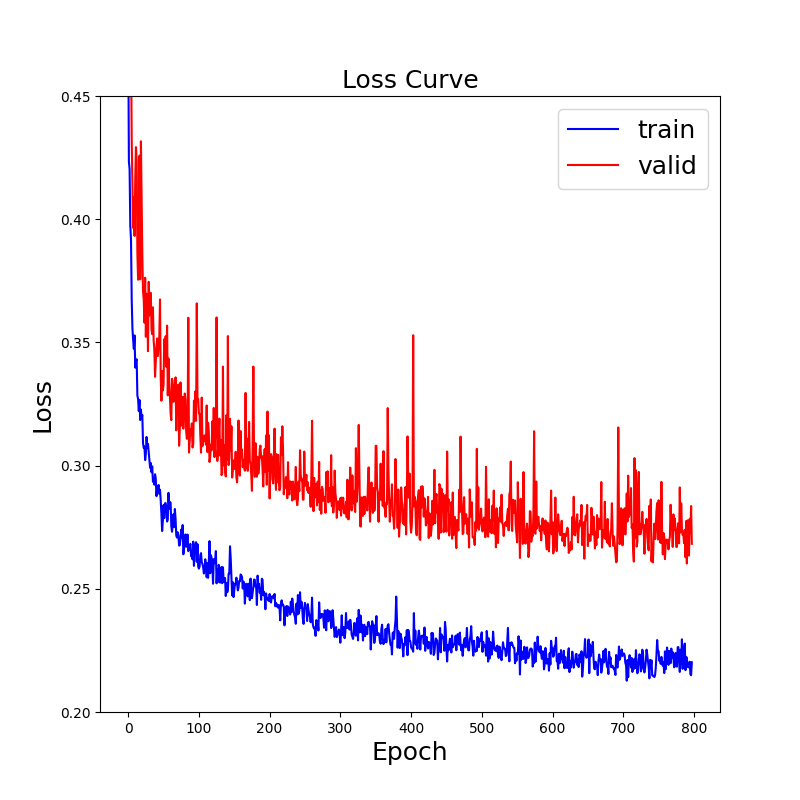
\includegraphics[width=12.0cm]{figures/loss_curve.png}
        \caption{Lovasz-Loss Curve}
        \label{loss_curve}
        \end{center}
\end{figure}
コンテストで提供される学習用画像2243枚の8割を学習用,2割を検証用に分割し学習を行った.
学習した際の学習曲線を図\ref{loss_curve}に示す.
解像度480*960の画像に対してGPU上で推論を行った結果,mIoUスコアは0.62となり,Lovasz-Loss関数を使用したことで精度が大幅に向上した.
\begin{table}[b]
    \caption{損失関数によるmIoUスコア比較} \vspace{1mm}
    \begin{center}
        \begin{tabular}{lc}
            SoftmaxWithCrossEntropy & 0.5093                     \\ \hline
            Lovasz Loss             & 0.6224
        \end{tabular}
    \end{center}
\end{table}